\documentclass[10pt]{article}
\usepackage{icmlko}

\icmlmeta{IP 파운데이션 월드모델}{89}{기획서를 넣으면 자리가 나온다}{도구를 만들었다 --- 그리고 기획서 열 칸 중 다섯을 모델이 안 쓴다는 것이 드러났다}

\begin{document}

\twocolumn[
\icmlheader

\begin{abstract}
모델 쪽 지렛대가 다 닫혔다 --- 배선(노트 76) · 부분집합(80) · 도메인 제거(82) ·
도메인 추가(83) · 구조(85--88). \textbf{남은 일은 쓸 수 있게 만드는 것이라
도구를 만들었다.} \texttt{state/score.py} 는 노트 77의 가장 엄격한 규약을 그대로
쓴다 --- 지금까지 연 팝업의 \emph{축만으로} 공간을 만들고, 새 기획 \emph{한 장}을
투영하고, 아홉 출처의 예측을 순위 평균해 \textbf{과거 팝업들 사이에서의 자리}를
낸다. 자기 검사를 붙였다 --- 과거 75건을 하나씩 빼고 매기면
\textbf{$\rho=+$0.4713}이다. 예시로 강한 기획이 상위 4\%(비슷한 자리의 과거
중앙 813명), 약한 기획이 상위 96\%(중앙 146명)로 갈린다. \textbf{도구를 만들자
드러난 것이 하나 있다} --- 기획서 열 속성 중 \textbf{다섯을 모델이 안 쓴다}.
체험 밀도 · 포토존 · 컬래버 강도 · IP 인지도 · 계절 적합은 팝업에만 있어 다른
도메인과 맞출 자리가 없다(노트 54에서 넣어 봤다가 $-$0.017). 그중 \textbf{IP
인지도는 대응물이 있다} --- 노트 84의 직전작 성적이 ``이 창작자/IP가 전에
얼마나 됐나''로 같은 것을 잰다. 넷째 공통 축으로 넣어 봤다. 판정치는 $+$0.4038에서
$+$0.4150으로 오르는데 \textbf{팝업은 $+$0.4501에서 $+$0.3992로 내린다.}
채택하지 않는다. \textbf{도구는 지금 상태로 쓸 수 있고, 기획서의 절반은 여전히
못 쓴다.}
\end{abstract}
]

\begin{figure*}[t]
\centering
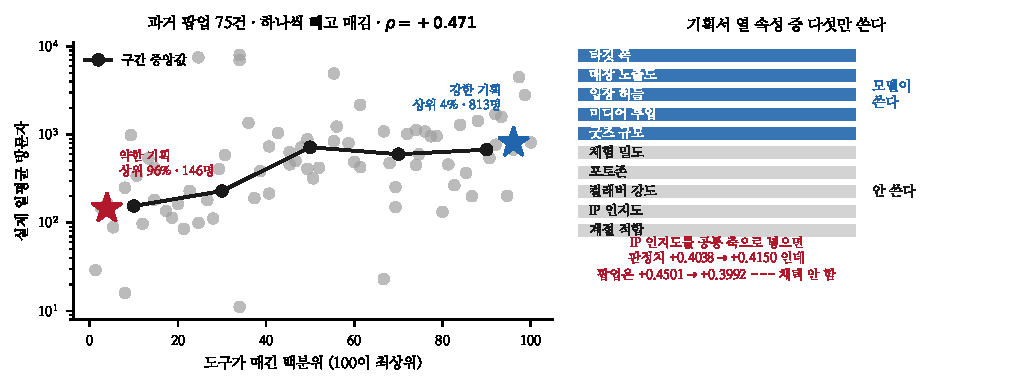
\includegraphics[width=\textwidth]{figs/tool.pdf}
\caption{왼쪽 --- 과거 팝업 75건의 자기 검사. 오른쪽 --- 쓰는 축과 안 쓰는 축.}
\end{figure*}

\section{도구}

\begin{quote}\fontsize{9.0}{11}\selectfont\ttfamily
python3 -m state.score --demo\\
python3 -m state.score --plan plan.json\\
python3 -m state.score --selftest
\end{quote}

규약은 노트 77의 규약 ④ 그대로다.

\begin{enumerate}[leftmargin=1.3em,itemsep=0.1em]
\item 지금까지 연 팝업의 \textbf{축만으로} 인자 공간을 만든다(라벨 안 씀)
\item 새 기획 \textbf{한 장}을 그 공간에 투영한다
\item 아홉 출처 도메인에서 각각 회귀를 학습해 예측한다
\item 순위 평균으로 합쳐 \textbf{과거 팝업들 사이의 자리}를 낸다
\end{enumerate}

\begin{table}[t]
\centering\tsize
\caption{예시 두 건.}
\begin{tabular}{lrr}
\toprule
& 강한 기획 & 약한 기획 \\
\midrule
자리 & \textbf{상위 4\%} & 상위 96\% \\
비슷한 자리 중앙 & 813명 & 146명 \\
비슷한 자리 범위 & 202--4,481 & 16--987 \\
\bottomrule
\end{tabular}
\end{table}

\claimx{도구가 과거 팝업 75건을 하나씩 빼고 매기면 $\rho=+$0.4713이다. 실제
쓰이는 방식(지금까지 연 것으로 공간을 만들고 새 기획 하나를 넣는다)과 같은
계산이므로 이 수가 도구의 성적이다.}{노트 77이 미래 팝업 59건에서 낸 $+$0.5268과
다르다. 표본이 달라서다(75건 전체 대 2025년 이후 59건). 둘 다 같은 규약이다.}

\paragraph{내는 것과 안 내는 것}
도구는 \textbf{순위}를 낸다. ``몇 명 올 것이다''는 안 낸다 --- 상하위 20\%의
방문자 배수가 7.6배인데 그 구간이 $[$1.8, 14.5$]$다(노트 76). 출력에 그
경고를 붙여 놨다.

\section{도구가 드러낸 것}

\begin{table}[t]
\centering\tsize
\caption{기획서 열 속성.}
\begin{tabular}{ll}
\toprule
\textbf{모델이 쓴다} & 타깃 폭 · 매장 노출도 · 입장 허들 \\
 & 미디어 투입 · 굿즈 규모 \\
\midrule
\textbf{안 쓴다} & 체험 밀도 · 포토존 · 컬래버 강도 \\
 & \textbf{IP 인지도} · 계절 적합 \\
\bottomrule
\end{tabular}
\end{table}

기획자가 채우는 열 칸 중 다섯을 모델이 버린다. 이유는 구조적이다 ---
\textbf{다른 도메인에 대응물이 없어 정렬에 못 쓴다}. 노트 36이 그런 축을 ``고유
축''으로 부르고 노트 54가 팝업에 넣어 봤다가 $-$0.017로 뺐다.

\begin{quote}\fontsize{9.5}{11.5}\selectfont
\textbf{그런데 IP 인지도는 다르다.} 다른 도메인에도 ``이 창작자/IP가 전에 얼마나
됐나''가 있다 --- 노트 84의 \textbf{직전작 성적}이 정확히 그것이며 모바일에서
단일 상관 $+$0.709를 냈다. 둘을 같은 슬롯에 넣으면 \textbf{네 번째 공통 축}이
된다.
\end{quote}

\begin{table}[t]
\centering\tsize
\caption{IP 인지도 $\leftrightarrow$ 직전작 성적을 한 슬롯에.}
\begin{tabular}{lrr}
\toprule
& 판정치 & 팝업 \\
\midrule
현행 & $+$0.4038 & \textbf{$+$0.4501} \\
공통 4축(중립 대입) & \textbf{$+$0.4150} & $+$0.3992 \\
고유 축(중립 대입) & $+$0.4130 & $+$0.4194 \\
공통 4축(마스크 유지) & $+$0.3997 & $+$0.4136 \\
\bottomrule
\end{tabular}
\end{table}

\claimx{IP 인지도와 직전작 성적을 한 슬롯에 넣으면 판정치가 $+$0.0112 오르는데
\textbf{팝업은 $-$0.0509 내린다}. 채택하지 않는다 --- 제품 목표가 내려가는
변경은 판정치가 올라도 못 쓴다.}{노트 75가 보였듯 팝업 75건으로는 $-$0.05를
잡음과 못 가른다. ``내렸다''도 확정이 아니다 --- 다만 오르지 않은 것은 확실하다.}

이것으로 노트 84가 연 실마리가 닫힌다. 직전작 성적은 도메인 안에서 가장 센
단일 변수인데(모바일 $+$0.709), 인자 공간에 넣는 세 가지 방법(고유 축 · 결측
표시자 · 공통 축)이 모두 문턱을 못 넘었다.

\section{한계}

\begin{itemize}[leftmargin=1.1em,itemsep=0.15em]
\item 도구가 쓰는 축이 다섯뿐이다. 기획자가 채운 절반이 버려진다.
\item ``비슷한 자리의 과거 팝업 방문자''는 백분위 근방 9건의 범위다.
      예측 구간이 아니라 \textbf{참고용 사례}다.
\item 자기 검사 $\rho=+$0.4713은 과거 75건 전체다. 시간을 가른 수치는
      노트 77의 $+$0.5268이다.
\item 도구가 팝업 도메인에만 쓸 수 있다. 다른 카테고리에 붙이려면 그 카테고리의
      과거 레코드가 최소 열몇 건 있어야 한다.
\item IP 인지도 실험에서 ``팝업이 내렸다''를 확정할 수 없다(표본 75건).
\end{itemize}

\section{다음}

\begin{enumerate}[leftmargin=1.3em,itemsep=0.15em]
\item \textbf{안 쓰는 다섯 축의 대응물을 다른 도메인에서 찾는다} --- 포토존은
      ``사진 찍을 거리''이고 체험 밀도는 ``할 일의 양''이다. 게임의 기능 수,
      웹툰의 회차, 애니의 러닝타임이 후보다.
\item 도구를 다른 카테고리로 넓힌다 --- 웹툰 · 만화 신작 기획에도 같은 규약이
      그대로 쓰인다.
\item 팝업 표본. 세 노트가 같은 곳을 가리킨다(75 · 86 · 87).
\item 열한째 도메인 --- 정밀도가 필요할 때만(노트 83).
\end{enumerate}

\vspace{0.6em}
\hrule height 0.3pt
\vspace{0.5em}
{\footnotesize
\textbf{참고문헌}\\[0.3em]
Ben-David, S. et al. (2010). A theory of learning from different domains.
\emph{Machine Learning}, 79(1--2), 151--175.\\[0.15em]
Schoenemann, P. H. (1966). A generalized solution of the orthogonal Procrustes
problem. \emph{Psychometrika}, 31(1), 1--10.\\[0.15em]
Little, R. J. A., Rubin, D. B. (2019). \emph{Statistical Analysis with Missing
Data}, 3rd ed. Wiley.\\[0.15em]
Kish, L. (1965). \emph{Survey Sampling}. Wiley.\\[0.15em]
Efron, B., Tibshirani, R. J. (1993). \emph{An Introduction to the Bootstrap}.
Chapman \& Hall.
}

\end{document}
